%%%%%%%%%%%%%%%%%%%%%%%%%%%%%%%%%%%%%%%%%
% Beamer Presentation
% LaTeX Template
% Version 1.0 (10/11/12)
%
% This template has been downloaded from:
% http://www.LaTeXTemplates.com
%
% License:
% CC BY-NC-SA 3.0 (http://creativecommons.org/licenses/by-nc-sa/3.0/)
%
%%%%%%%%%%%%%%%%%%%%%%%%%%%%%%%%%%%%%%%%%

%----------------------------------------------------------------------------------------
%	PACKAGES AND THEMES
%----------------------------------------------------------------------------------------

\documentclass{beamer}

\mode<presentation> {

% The Beamer class comes with a number of default slide themes
% which change the colors and layouts of slides. Below this is a list
% of all the themes, uncomment each in turn to see what they look like.

%\usetheme{default}
%\usetheme{AnnArbor}
%\usetheme{Antibes}
%\usetheme{Bergen}
%\usetheme{Berkeley}
%\usetheme{Berlin}
%\usetheme{Boadilla}
%\usetheme{CambridgeUS}
%\usetheme{Copenhagen}
%\usetheme{Darmstadt}
%\usetheme{Dresden}
%\usetheme{Frankfurt}
%\usetheme{Goettingen}
%\usetheme{Hannover}
%\usetheme{Ilmenau}
%\usetheme{JuanLesPins}
%\usetheme{Luebeck}
\usetheme{Madrid}
%\usetheme{Malmoe}
%\usetheme{Marburg}
%\usetheme{Montpellier}
%\usetheme{PaloAlto}
%\usetheme{Pittsburgh}
%\usetheme{Rochester}
%\usetheme{Singapore}
%\usetheme{Szeged}
%\usetheme{Warsaw}

% As well as themes, the Beamer class has a number of color themes
% for any slide theme. Uncomment each of these in turn to see how it
% changes the colors of your current slide theme.

%\usecolortheme{albatross}
%\usecolortheme{beaver}
%\usecolortheme{beetle}
%\usecolortheme{crane}
%\usecolortheme{dolphin}
%\usecolortheme{dove}
%\usecolortheme{fly}
%\usecolortheme{lily}
%\usecolortheme{orchid}
%\usecolortheme{rose}
%\usecolortheme{seagull}
%\usecolortheme{seahorse}
%\usecolortheme{whale}
%\usecolortheme{wolverine}

%\setbeamertemplate{footline} % To remove the footer line in all slides uncomment this line
%\setbeamertemplate{footline}[page number] % To replace the footer line in all slides with a simple slide count uncomment this line

%\setbeamertemplate{navigation symbols}{} % To remove the navigation symbols from the bottom of all slides uncomment this line
}

\usepackage{graphicx} % Allows including images
\usepackage{booktabs} % Allows the use of \toprule, \midrule and \bottomrule in tables
\usepackage{amssymb}
\usepackage{mathtools}
\usepackage{pdfpages}
\usepackage[utf8]{inputenc}


%----------------------------------------------------------------------------------------
%	TITLE PAGE
%----------------------------------------------------------------------------------------

\title[GAN]{Generative Adversarial Networks} % The short title appears at the bottom of every slide, the full title is only on the title page

\author{Bruno Gavranović} % Your name
\institute[PSIML2017] % Your institution as it will appear on the bottom of every slide, may be shorthand to save space
{
Petnica Summer School of Machine Learning\\ % Your institution for the title page
\medskip
\textit{bruno.gavranovic@fer.hr} % Your email address
}
\date{\today} % Date, can be changed to a custom date
\graphicspath{{img/}}
\begin{document}

\begin{frame}
\titlepage % Print the title page as the first slide
\end{frame}

\begin{frame}
\frametitle{Overview} % Table of contents slide, comment this block out to remove it
\tableofcontents % Throughout your presentation, if you choose to use \section{} and \subsection{} commands, these will automatically be printed on this slide as an overview of your presentation
\end{frame}

%----------------------------------------------------------------------------------------
%	PRESENTATION SLIDES
%----------------------------------------------------------------------------------------

%------------------------------------------------
\section{Meta} % Sections can be created in order to organize your presentation into discrete blocks, all sections and subsections are automatically printed in the table of contents as an overview of the talk
%------------------------------------------------

\subsection{Subsection Example} % A subsection can be created just before a set of slides with a common theme to further break down your presentation into chunks

\begin{frame}
\frametitle{Meta}
\begin{itemize}
	\item What is this talk about?
	\item Unlike the most of the things you will be learning in this course, this model is new
	\item New idea
	\item Nobody is still sure how it works
	\item Compared to other ML models, we're still in early stages
	\item Our understanding of it changes from week to week
\end{itemize}
\begin{block}{Yann LeCun}
"The most important one, in my opinion, is adversarial training (also called GAN for Generative Adversarial Networks).

This, and the variations that are now being proposed is the most interesting idea in the last 10 years in ML, in my opinion.”
\end{block}
\end{frame}

%------------------------------------------------

\begin{frame}
\begin{figure}[h!]
	\centering
	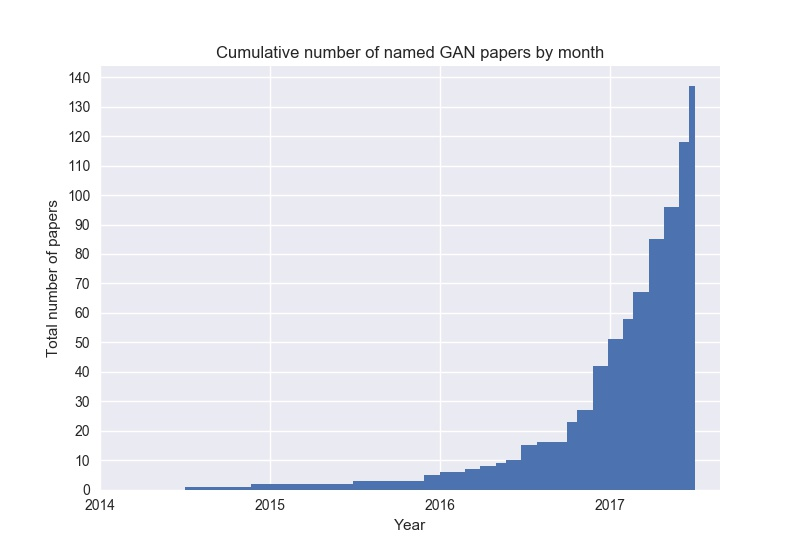
\includegraphics[width=0.95\textwidth]{gan_timeline.jpg}
	\caption{GAN timeline}
	\label{fig:gan_timeline}
\end{figure}

\end{frame}

%------------------------------------------------

\begin{frame}
	\frametitle{GAN: Just tell me what it is}
	\begin{itemize}
		\item Generative machine learning model in which two neural networks are competing against each other
	\end{itemize}
\begin{figure}[h!]
	\centering
	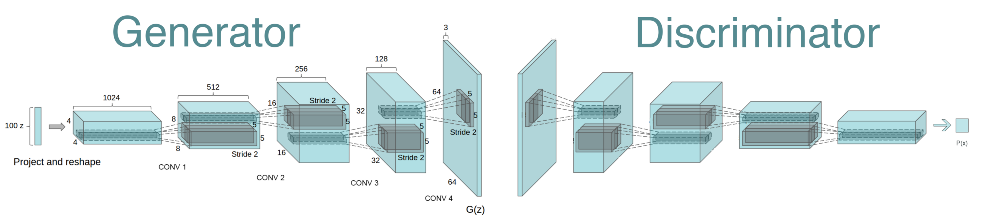
\includegraphics[width=\textwidth]{dcgan_both.png}
\end{figure}
	\begin{itemize}
		\item Instead of using a standard fixed cost function, we \textit{learn} the cost function with the neural network
		\item We alternate between training different parts of the network
		\item It's difficult to train and analyze
	\end{itemize}
\footnotetext{https://github.com/dmonn/GAN-face-generator}
\end{frame}

\begin{frame}
\begin{figure}[h!]
	\centering
	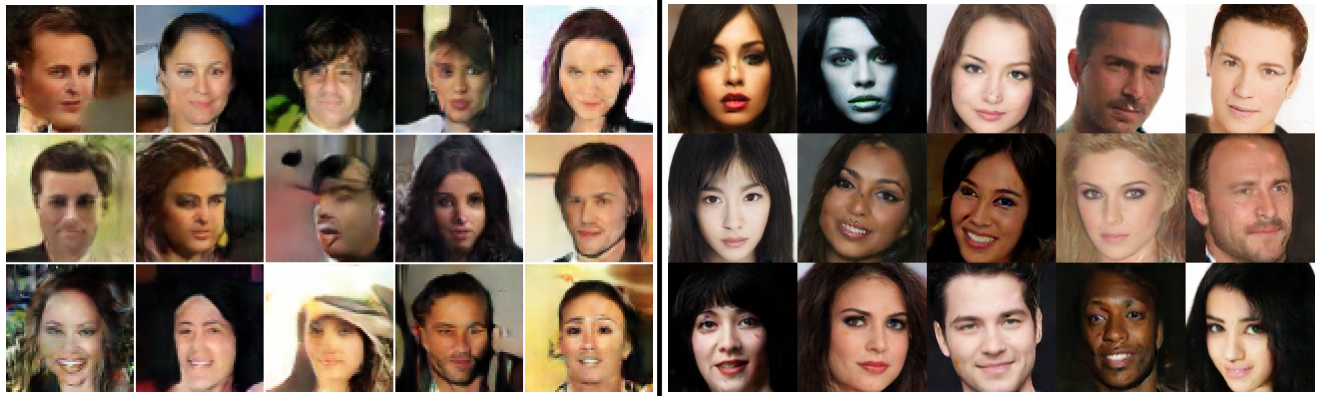
\includegraphics[width=\textwidth]{which_is_real.png}
	\caption{Which side are real images?}
	\label{fig:which_is_real}
\end{figure}
\end{frame}


%------------------------------------------------
\begin{frame}
\begin{figure}[h!]
	\centering
	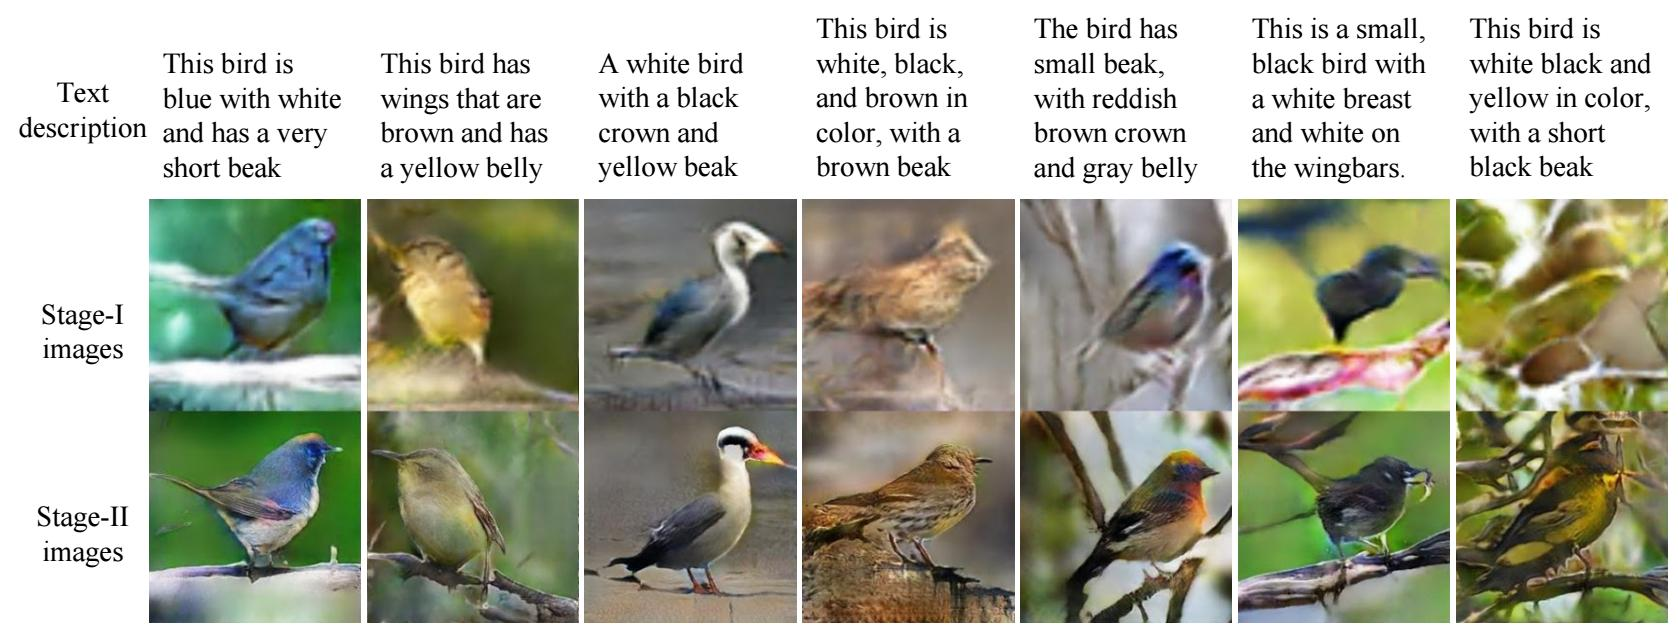
\includegraphics[width=\textwidth]{stack_gan.jpg}
	\caption{StackGAN}
\end{figure}
\end{frame}

\begin{frame}
\begin{figure}[h!]
	\centering
	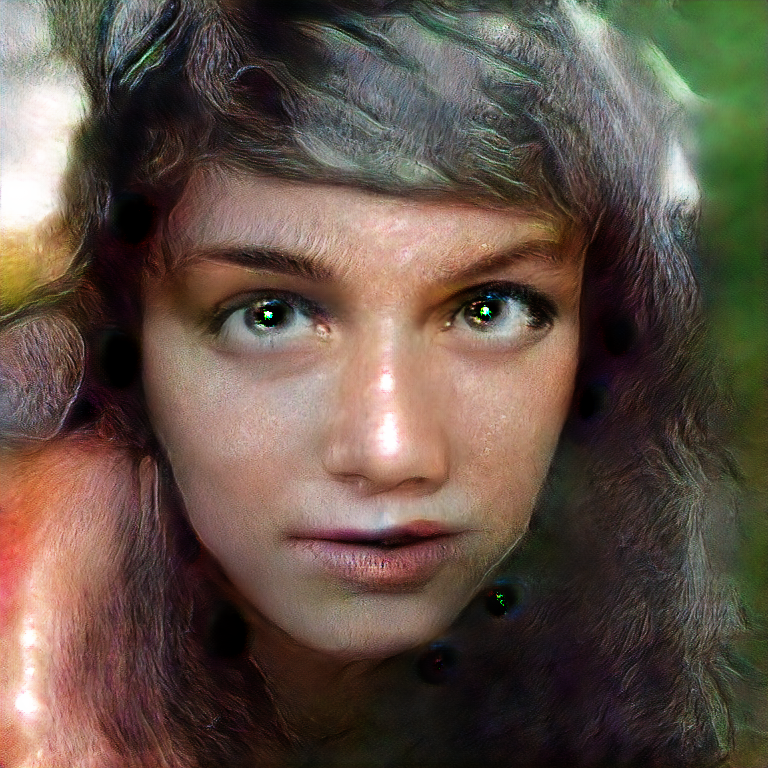
\includegraphics[width=0.8\textwidth]{4k_woman.jpg}
\end{figure}
\end{frame}

\begin{frame}
\begin{figure}[h!]
	\centering
	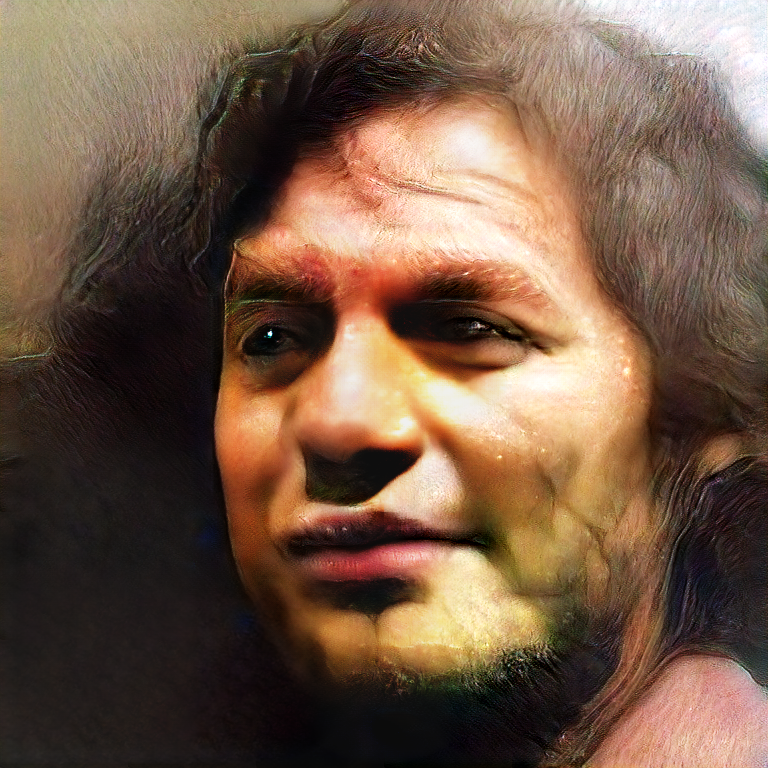
\includegraphics[width=0.8\textwidth]{4k_man.jpg}
\end{figure}
\end{frame}

\begin{frame}
\begin{figure}[h!]
	\centering
	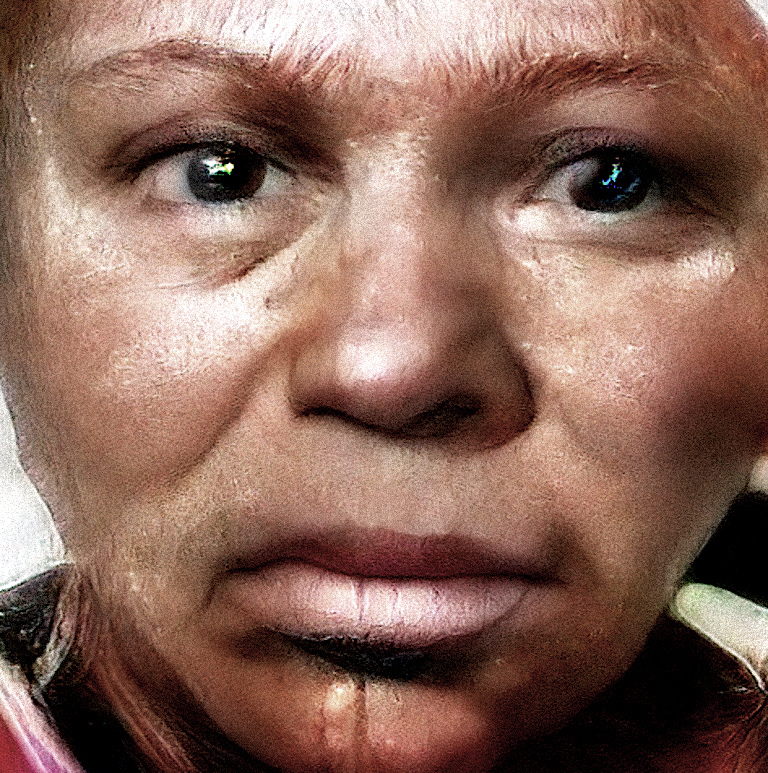
\includegraphics[width=0.8\textwidth]{4k_black_woman.jpg}
\end{figure}
\end{frame}
%------------------------------------------------
\begin{frame}
\frametitle{What is this talk about?}
\begin{itemize}
	\item Theory behind Generative Adversarial Networks
	\item Comparison of different models
	\item Practical advice for training
	\item Everything is a Work In Progress.
\end{itemize}

\end{frame}


\section{Prerequisites}


\begin{frame}
\frametitle{Prerequisites}
\begin{itemize}
	\item Understanding real world data
	\item Natural data forms a low dimensional manifold in its embedding space
\end{itemize}
\begin{figure}[h!]
	\centering
	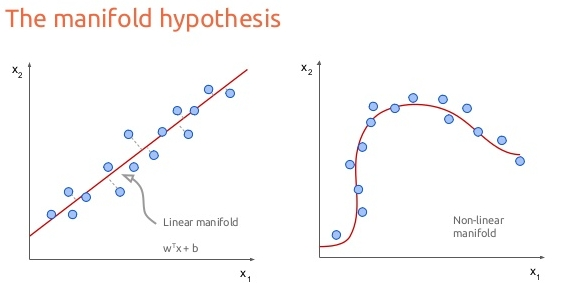
\includegraphics[width=0.8\textwidth]{manifold_hypothesis.jpg}
\end{figure}

\end{frame}
\begin{frame}
\begin{figure}[h!]
	\centering
	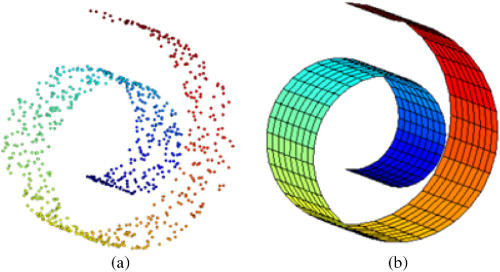
\includegraphics[width=0.8\textwidth]{swiss_roll.jpg}
\end{figure}

\end{frame}

\begin{frame}
\begin{figure}[h!]
	\centering
	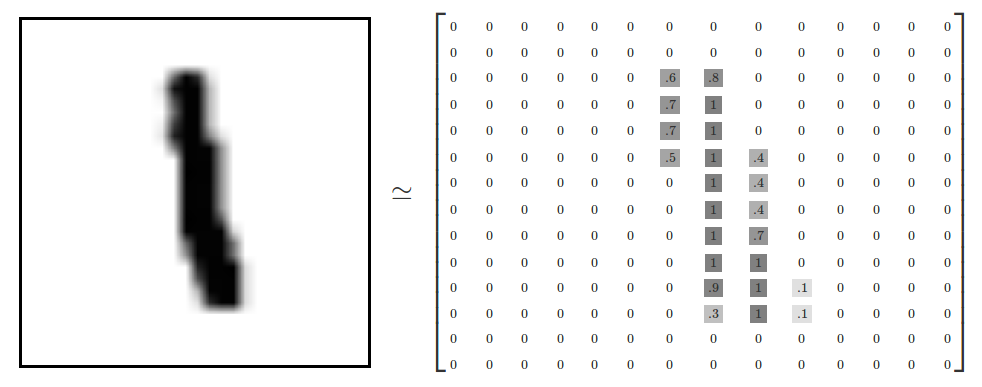
\includegraphics[width=\textwidth]{mnist_pixel_space.png}
\end{figure}

\end{frame}

\begin{frame}
\begin{figure}[h!]
	\centering
	\includegraphics<1>[width=\textwidth]{distr/1.png}
	\includegraphics<2>[width=\textwidth]{distr/2.png}
	\includegraphics<3>[width=\textwidth]{distr/3.png}
	\includegraphics<4>[width=\textwidth]{distr/4.png}
	\includegraphics<5>[width=\textwidth]{distr/5.png}
	\includegraphics<6>[width=\textwidth]{distr/6.png}
	\includegraphics<7>[width=\textwidth]{distr/7.png}
\end{figure}
\end{frame} 

\section{Basic principles}

\begin{frame}
\frametitle{Distribution matching}
	\begin{itemize}
		\item We have parameters $\theta$
		\item We can define a parametric function $g_\theta$ that generates samples from a certain distribution $\mathbb{P}_\theta$
		\item We have samples from the real data distribution $\mathbb{P}_\textit{r}$
		\item By varying weights of the neural network we can make the $\mathbb{P}_\theta$ distribution arbitrarily close to $\mathbb{P}_\textit{r}$
		\item How do we define ``close"?
\end{itemize}
\end{frame}

\begin{frame}
\frametitle{First attempt}
\begin{columns}
\begin{column}{0.5\textwidth}
\begin{itemize}
	\item How to match the distributions?
\end{itemize}
\end{column}
\begin{column}{0.5\textwidth}  %%<--- here
\begin{figure}[h!]
	\centering
	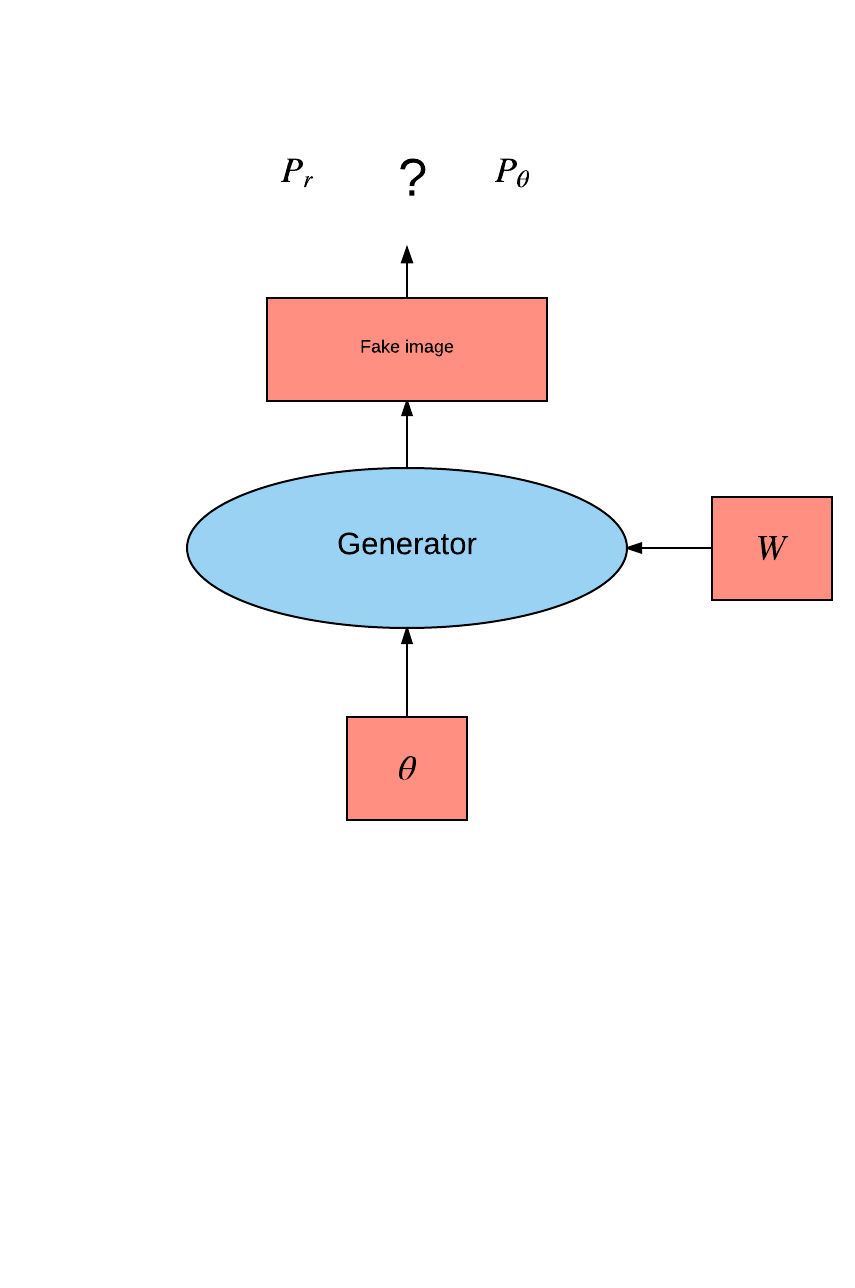
\includegraphics[width=0.8\textwidth]{first_attempt_gan.png}
\end{figure}
\end{column}
\end{columns}


\end{frame}

\begin{frame}
\frametitle{First attempt}
\begin{columns}
\begin{column}{0.5\textwidth}
\begin{itemize}
	\item Trying to recreate existing images
	\item Encoding the images into the bottleneck $\theta$
	\item Implicitly training the network to extract useful features
\end{itemize}
\end{column}
\begin{column}{0.5\textwidth}  %%<--- here
\begin{figure}[h!]
	\centering
	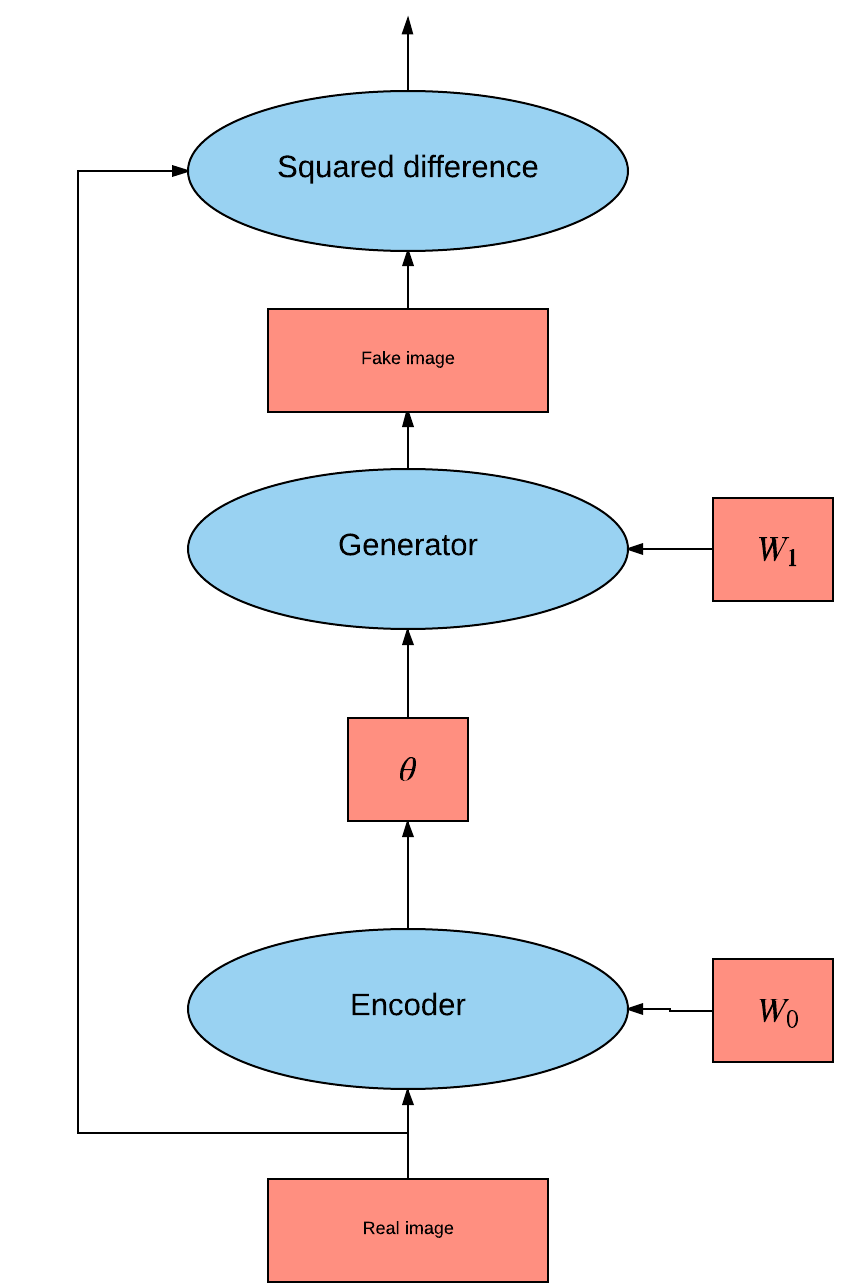
\includegraphics[width=0.8\textwidth]{autoencoder_attempt.png}
\end{figure}
\end{column}
\end{columns}

\end{frame}

%------------------------------------------------
\begin{frame}
\begin{figure}[h!]
	\centering
	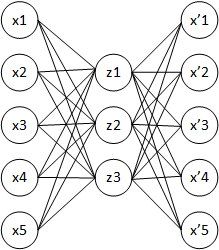
\includegraphics[width=0.5\textwidth]{autoencoder_bad_diagram.png}
\end{figure}

\end{frame}
%------------------------------------------------
\begin{frame}
	\frametitle{Core principles}
	\begin{itemize}
		\item Neural network is a computational graph!
		\item Backpropagation is reverse-mode automatic differentiation
		\item Decomposing the network into basic building blocks
	\end{itemize}
\end{frame}

%------------------------------------------------
\begin{frame}
\begin{columns}
\begin{column}{0.5\textwidth}
	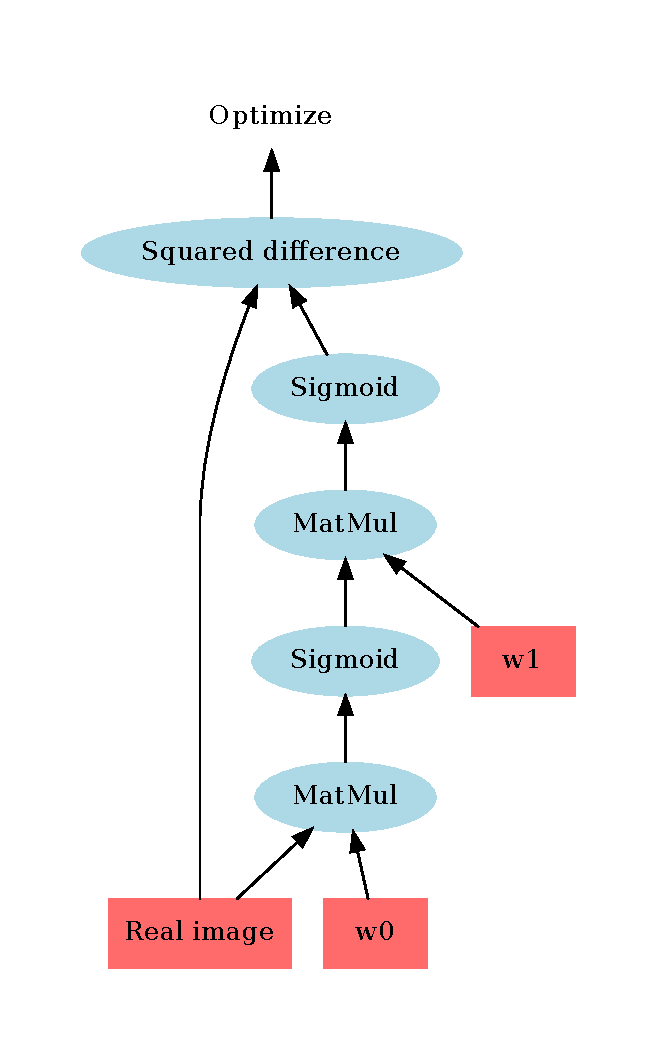
\includegraphics[width=\textwidth]{sq_diff.pdf}
	\pause
\end{column}
\begin{column}{0.5\textwidth}  %%<--- here
	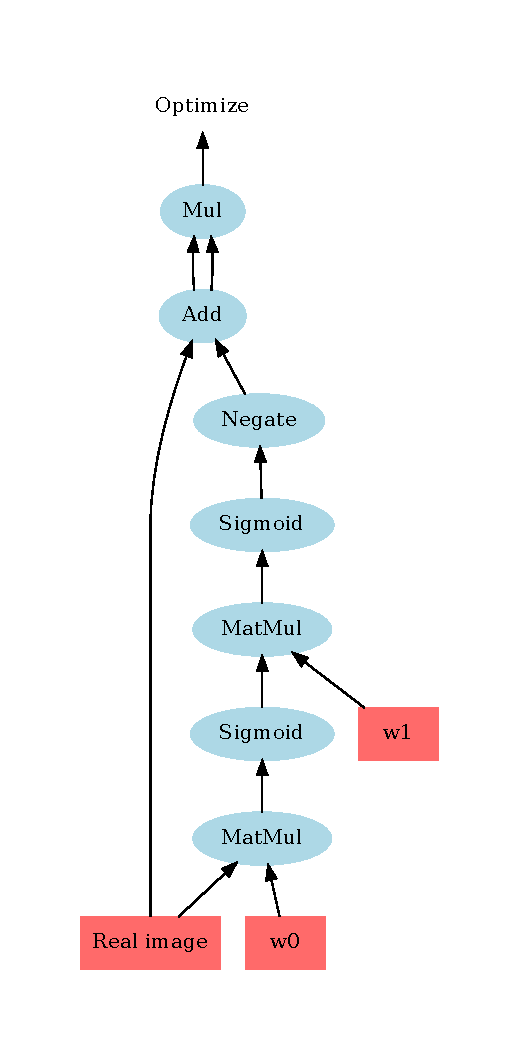
\includegraphics[width=0.8\textwidth]{sq_diff_all.pdf}
\end{column}
\end{columns}
\end{frame}
%------------------------------------------------
\begin{frame}
\begin{columns}
\begin{column}{0.5\textwidth}
	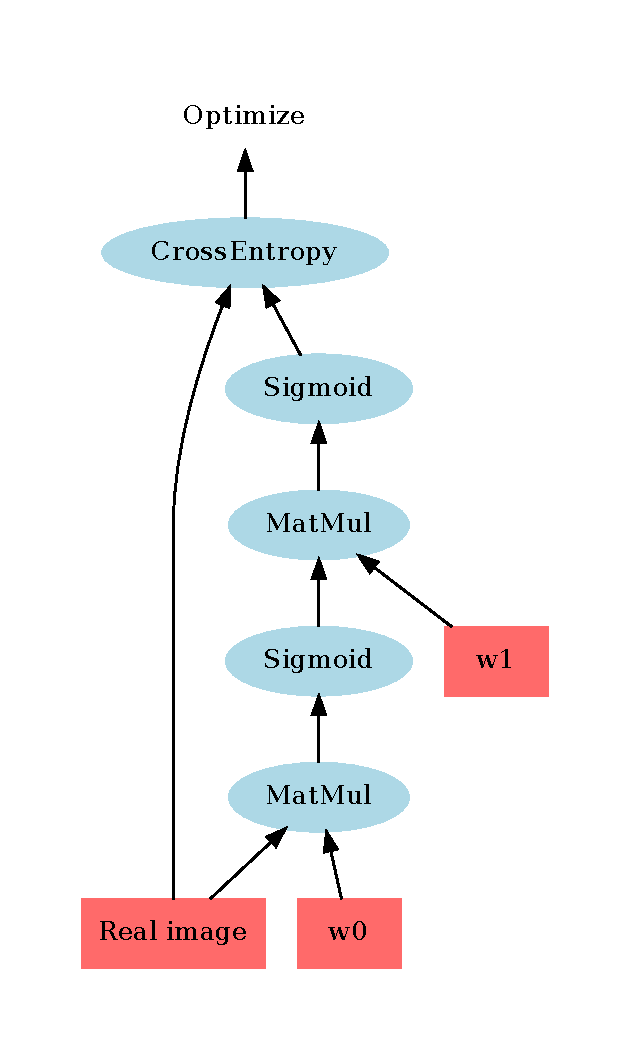
\includegraphics[width=\textwidth]{cross_entropy.pdf}
	\pause
\end{column}
\begin{column}{0.5\textwidth}  %%<--- here
	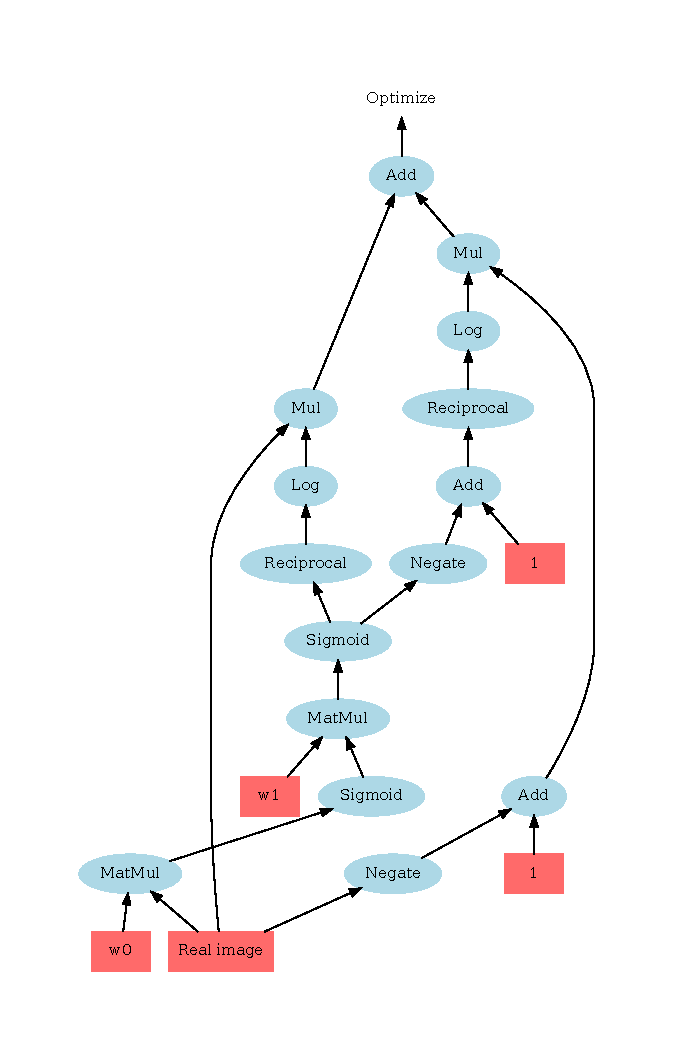
\includegraphics[width=\textwidth]{cross_entropy_all.pdf}
\end{column}
\end{columns}
\end{frame}

%------------------------------------------------
\begin{frame}
	\begin{figure}[h!]
	\centering
	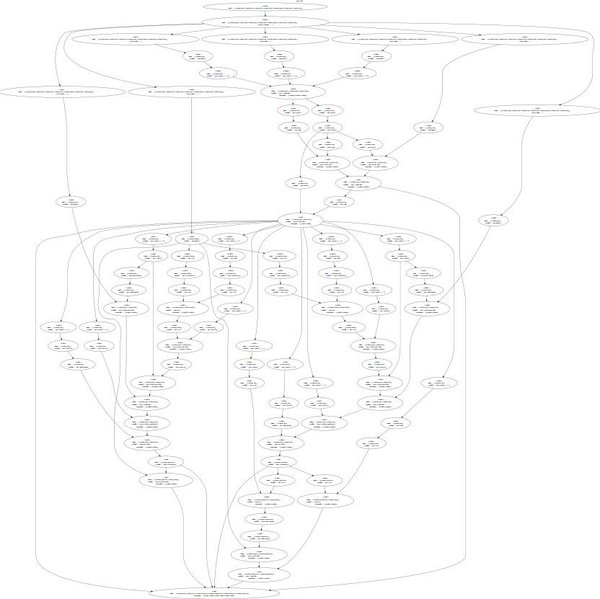
\includegraphics[width=0.6\textwidth]{ntm_comp_graph.jpg}
	\caption{Neural turing machines computational graph}
	\label{fig:ntm_comp_graph}
	\end{figure}

\end{frame}
%------------------------------------------------
\begin{frame}
	\frametitle{Things to note}
	\begin{itemize}
		\item Cost function is not parametrized (it's fixed)
		\item We train the network with just one cost function
		\item Weight freezing and sharing is fixed throughout the training
	\end{itemize}
\end{frame}

%------------------------------------------------
\begin{frame}
	\frametitle{Cost function}
	\begin{itemize}
		\item MSE needs to average over all possibilities and choose a single answer
		\item Square error - a simple parabola, is it sufficient?
	\end{itemize}
	\begin{figure}[h!]
		\centering
		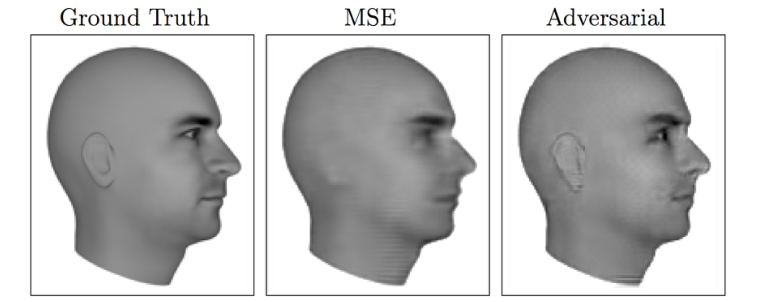
\includegraphics[width=\textwidth]{mse_vs_adversarial.png}
	\end{figure}
	\footnotetext{Ian J. Goodfellow:
NIPS 2016 Tutorial: Generative Adversarial Networks}
\end{frame}
%------------------------------------------------
\begin{frame}
	\frametitle{A common pattern}
	\begin{itemize}
		\item The great idea - why don't we put a neural network as the cost function?
		\item Introduces a lot of problems
		\item How do we even train this thing?
		\item How do we analyze it's behaviour?
	\end{itemize}
\end{frame}

%------------------------------------------------
\begin{frame}
	\frametitle{A common pattern}
	\begin{itemize}
		\item Standard NN with a cost function
		\item One phase of training GAN is the same 
		\item Other phase of GAN is training the cost function
	\end{itemize}
\end{frame}

%------------------------------------------------
\begin{frame}
	\frametitle{Modular training, different objectives}
	\begin{itemize}
		\item Usually we have a cost function and we backprop through the whole network and change all the weights
		\item GAN doesn't have just one cost function and it has different ways of backpropagating
		\item LSTM has weights fixed in every time step
		\item Convolutional network has weights fixed to form filters
		\item GAN has weights fixed during different parts of training
	\end{itemize}
\end{frame}

%------------------------------------------------

\begin{frame}
	\frametitle{A common pattern}
	\begin{itemize}
		\item Image with three different optimizations and ways of freezing weights
		\item It boils down to two different things we optimize
	\end{itemize}
\end{frame}

%------------------------------------------------
\begin{frame}
	\frametitle{Intuitive approach}
	\begin{itemize}
		\item Forger and the police
		\item Forger tries to create real looking money
		\item Police tries to get better at detecting fake money
		\item They both keep improving until the difference between fake and real money is imperceptible to us
	\end{itemize}
\end{frame}
%------------------------------------------------
\begin{frame}
	\frametitle{Different statistical distances}
	\begin{itemize}
		\item Defining distance between two points in Euclidean space is intuitive
		\item How do we define distances between distributions?
		\item Recall from before - we have real and fake images, we want fake distribution to become same as real
		\item Instead of comparing distributions in the pixel space - we use the neural network (the cost function) to transform them to a more suitable representation
		\item But we still have to compare those distributions
	\end{itemize}
\end{frame}
%------------------------------------------------
\begin{frame}
	\frametitle{Various statistical distances - divergences}
	\begin{itemize}
		\item KL-divergence
		\item JS-divergence
		\item Earth-mover distance (Wasserstein distance)
		\item Total variation distance
		\item ...
	\end{itemize}
\end{frame}
%------------------------------------------------
\begin{frame}
	\frametitle{KL-divergence}
	\begin{exampleblock}{KL-divergence}
	\[
		KL(\mathbb{P} \vert \vert \mathbb{Q}) = \mathbb{E}_{x \sim \mathbb{P}} \Big[ \log \frac{P(x)}{Q(x)} \Big] = \int_{x} \log \frac{P(x)}{Q(x)} P(x) dx
	\]
\end{exampleblock}
	\begin{itemize}
		\item Doesn't satisfy triangle inequality and symmetry
		\item Origins in information theory
		\item Information gained when revising from prior Q to posterior P
		\item Originally proposed by Goodfellow \textit{et al.} as the function to compute ``distance" with
		\item Has some undesirable properties
	\end{itemize}
\end{frame}

%------------------------------------------------
\begin{frame}
	\frametitle{History of training GANs with KL}
	\begin{itemize}
		\item Very unstable
		\item We're training the cost function at the same time as the generator - we want the cost function to be as good as possible
		\item But we can't train it to be \textit{too good} since the gradients computed with KL will vanish
		\item Why? Because distributions have low dimensional support and KL does to infinity when Q is zero
		\item Requires careful tuning of hyperparameters and has the "it works but we don't know why" philosophy
		\item Difficult to train
		\item Loss doesn't correlate with image quality
	\end{itemize}
\end{frame}

%------------------------------------------------
\begin{frame}
	\frametitle{Wasserstein (Earth mover) distance}
	\begin{exampleblock}{EM distance}
	\[
		W(\mathbb{P}, \mathbb{Q}) = \inf_{\gamma \in \Pi(\mathbb{P}, \mathbb{Q})} {\mathbb{E}_{(x, y) \sim \gamma}} \big[ \lvert \lvert x - y \lvert \lvert \big]
	\]
\end{exampleblock}
	\begin{itemize}
		\item Distance function that takes into account underlying geometry of the distributions
		\item Minimum cost of turning a pile of dirt into the other
		\item Proposed by Arjovsky \textit{et al.} as improvement to original GAN training - Wasserstein GAN
	\end{itemize}
\end{frame}

%------------------------------------------------
\begin{frame}
	\frametitle{Learning distributions - toy example}
	\begin{columns}
	\begin{column}{0.5\textwidth}
	\begin{figure}[h!]
		\centering
		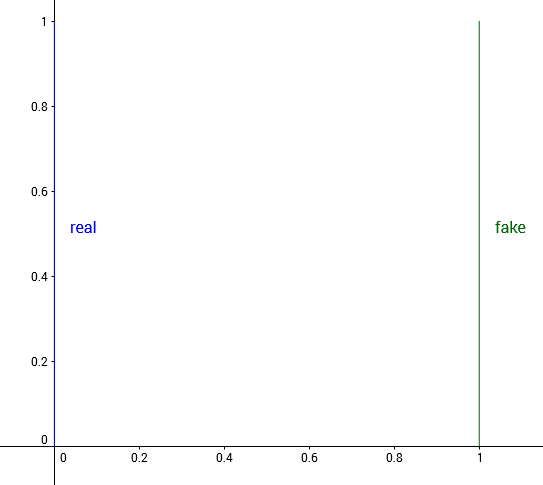
\includegraphics[width=0.9\textwidth]{two_lines.png}
	\end{figure}
	\pause
	$\mathbb{P}_r = (0, y) \quad \quad \quad \quad \quad \quad \mathbb{P}_g = (\theta, y)$
	\pause
	\begin{center}
		$y \sim U\big[0, 1\big]$
	\end{center}
	\end{column}
	\begin{column}{0.5\textwidth}  %%<--- here
	\pause
	\begin{itemize}
		\item Two distributions defined on $\mathbb{R}^2$
			\newline
		\pause
		\item  $ KL(\mathbb{P}_r \vert \vert \mathbb{P}_g) = +\infty$
		\pause
		\item  $ KL(\mathbb{P}_g \vert \vert \mathbb{P}_r) = +\infty$
		\pause
		\item  $ JS(\mathbb{P}_r, \mathbb{P}_g) = JS(\mathbb{P}_g, \mathbb{P}_r) = \log 2 $
		\pause
		\item  $ W(\mathbb{P}_r, \mathbb{P}_g) = W(\mathbb{P}_g, \mathbb{P}_r) = \vert \theta \vert $
	\end{itemize}
	\end{column}
	\end{columns}
	\footnotetext{http://www.alexirpan.com/2017/02/22/wasserstein-gan.html}
\end{frame}

%------------------------------------------------
\begin{frame}
	\frametitle{Game theory perspective}
	\begin{itemize}
		\item \textit{Competition} between the generator and the critic
		\item Nash equilibrium
	\end{itemize}
\end{frame}

%------------------------------------------------
\begin{frame}
	\frametitle{EMD - drawbacks}
	\begin{itemize}
		\item Can't really compare critics
		\item Can't tell how how close to EM distance our estimate really is
		\item KL-divergence, when parameters are right, seems to produce much better looking samples?
	\end{itemize}
\end{frame}

%------------------------------------------------
\begin{frame}
	\frametitle{A common pattern}
	\begin{itemize}
		\item
	\end{itemize}
\end{frame}
%------------------------------------------------
\begin{frame}
\frametitle{Perspectives}
\begin{itemize}
	\item Distribution matching
	\item Neural network as a cost function
	\item Modular training
	\item Two player minimax game
\end{itemize}
\end{frame}

%------------------------------------------------

\begin{frame}
	\frametitle{Problems with GANs}
	\begin{itemize}
		\item Problems with counting
		\item High level structure
		\item Perspective
		\item Sequential data
		\item 
	\end{itemize}
\end{frame}


%------------------------------------------------
\begin{frame}
	\frametitle{Open questions}
	\begin{itemize}
		\item Which statistical distance to use?
		\item Best training regime?
		\item Convergence conditions?
		\item 
		\item Where does the neural network end the cost function begin?
		\item We optimize computational graph, but it's constituents have different semantics
		\item How is the cost function different from a neural network layer?
	\end{itemize}
\end{frame}

%------------------------------------------------
\begin{frame}
\frametitle{History of great ideas in deep learning}

\begin{itemize}
	\item We have to do lots of feature engineering, but when we do, the model works!
	\item Oh, we can let the NN do it by itself. We still have to figure out the cost function though, but when we do, the model works!
	\item Oh, we can let GAN figure out the cost FN by itself. We still have to figure out which optimizer to use and how to make it work.
	\item Oh, we can let the NN optimize itself...?
	\item Learning to learn by gradient descent by gradient descent
\end{itemize}

\end{frame}

%------------------------------------------------


\begin{frame}
\Huge{\centerline{The End}}
\end{frame}

%----------------------------------------------------------------------------------------

\end{document}
